\documentclass[10pt, a4paper]{article}
\usepackage[utf8]{inputenc}
\usepackage[russian]{babel}
\usepackage[sb]{libertine}
\usepackage{a4wide}
\usepackage{listings}
\usepackage{graphicx} 

\begin{document}

\title{Отчёт по лабораторной работе №5}
\author{Окорочкова Мария, M32341}

\maketitle

Текущая конфигурация системы:

\begin{tabular}{|l|r|}
      \hline
    Общий объем оперативной памяти & \texttt{12Gi} \\
    Объем раздела подкачки & \texttt{4.0Gi} \\
    Объем свободной физической памяти в ненагруженной системе & \texttt{10Gi} \\
    Объем свободного пространства в разделе подкачки в ненагруженной системе & \texttt{2.5Gi} \\
    Размер страницы виртуальной памяти & \texttt{4096B} \\
    \hline
\end{tabular}

\section*{Эксперимент №1}

\subsection*{Первый этап}

\subsubsection*{Значения параметров mem.bash}

\begin{itemize}
    \item PID, USER, PR, NI, SHR, S и COMMAND очевидно не изменялись (в следующих пунтктах учитываем это по умолчанию)
    \item TIME+ очевидно росло равномерно (в следующих пунтктах учитываем это по умолчанию)
    \item \%MEM, \%CPU:

    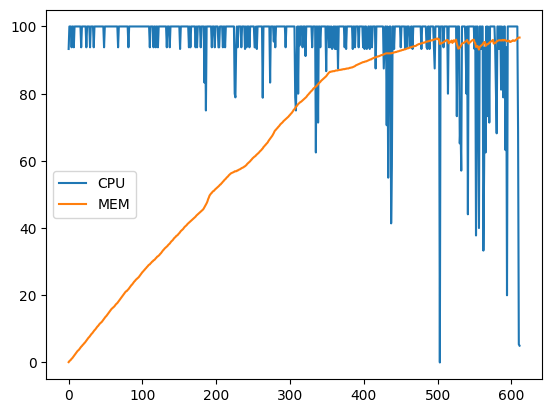
\includegraphics[scale=0.8]{graphs/1.png}
    \item VIRT, RES:
    
    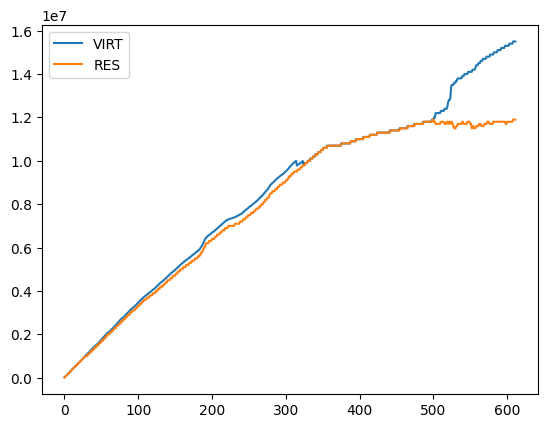
\includegraphics[scale=0.8]{graphs/2.png}
    \item free MEM, free SWAP:
    
    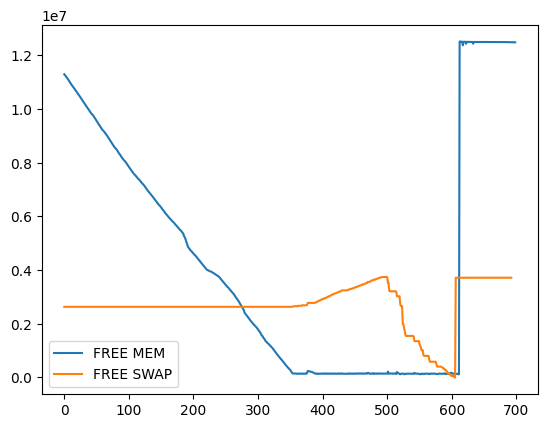
\includegraphics[scale=0.8]{graphs/3.png}
\end{itemize}

\textbf{dmesg | grep "mem.bash" : }
\begin{lstlisting}
[28872.410521] [  18073]  1000 18073  4064752  3118321 32620544   944342             0 mem.bash


[28872.410533] oom-kill:constraint=CONSTRAINT_NONE,nodemask=(null),cpuset=/,

mems_allowed=0,global_oom,task_memcg=/,task=mem.bash,pid=18073,uid=1000


[28872.411552] Out of memory: Killed process 18073 (mem.bash) total-vm:16259008kB, 

anon-rss:12473284kB, file-rss:0kB, shmem-rss:0kB, UID:1000 pgtables:31856kB 

oom_score_adj:0


[28873.006178] oom_reaper: reaped process 18073 (mem.bash), now anon-rss:0kB, 

file-rss:0kB, shmem-rss:0kB
\end{lstlisting}

Значение последней строки в файле \texttt{report.log} --- \textbf{208 000 000} --- примерно максимальный размер массива. Это мы запомним для второго эксперимента!

\textbf{Комментарий:}
Процесс убился, очевидно по всем графикам.

\subsection*{Второй этап}

\subsubsection*{Значения параметров mem[2]*.bash }

\begin{itemize}
    \item mem.bash \& mem2.bash: \%MEM, \%CPU:

    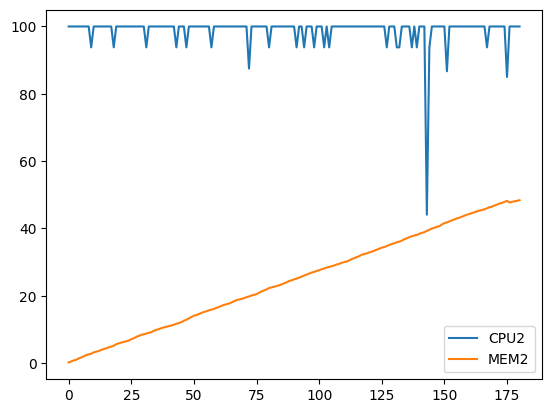
\includegraphics[scale=0.5]{graphs/5.png}
    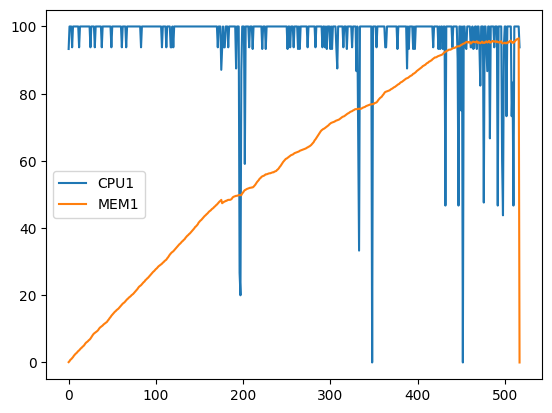
\includegraphics[scale=0.5]{graphs/4.png}
    \item mem.bash + mem2.bash: \%MEM, \%CPU:

    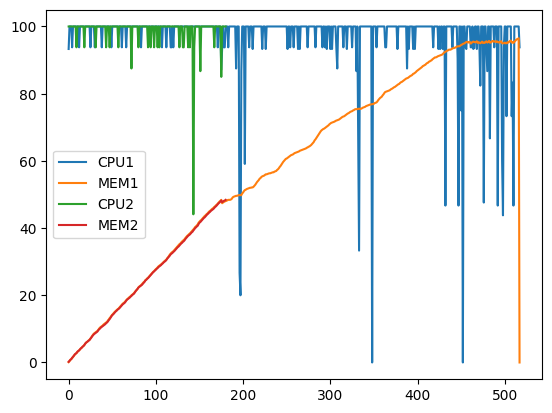
\includegraphics[scale=0.8]{graphs/6.png}
    \item mem.bash \& mem2.bash: VIRT, RES:

    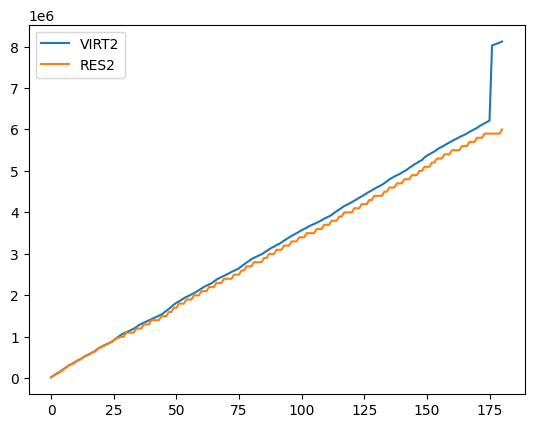
\includegraphics[scale=0.5]{graphs/8.png}
    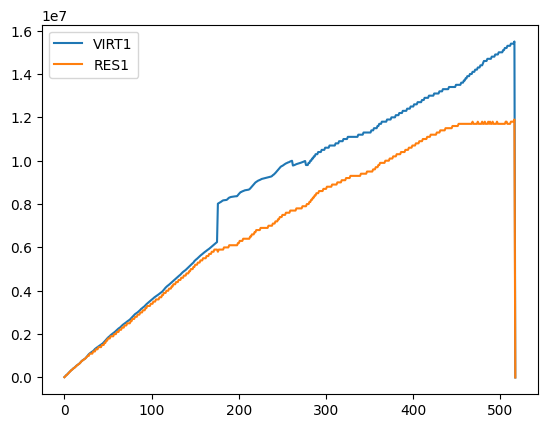
\includegraphics[scale=0.5]{graphs/7.png}
    \item mem.bash + mem2.bash: VIRT, RES:

    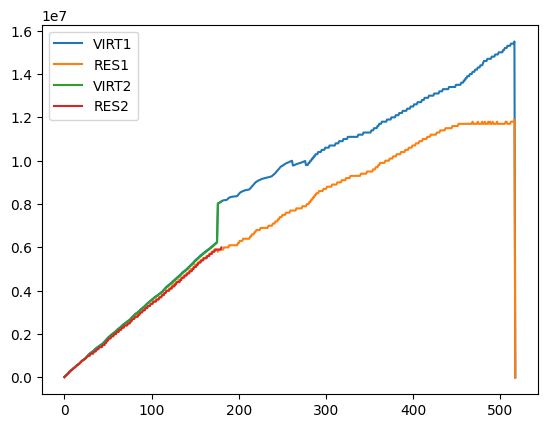
\includegraphics[scale=0.8]{graphs/9.png}
    \item free MEM, free SWAP:
    
    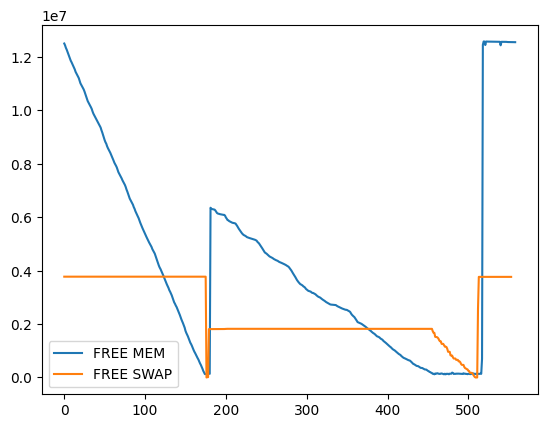
\includegraphics[scale=0.8]{graphs/10.png}
\end{itemize}

\textbf{dmesg | grep "mem[2]*.bash" :}
\begin{lstlisting}
[30613.250003] [   4884]  1000  4884  2032480  1556012 16334848   474371             0 mem.bash

[30613.250005] [   4885]  1000  4885  2032579  1563609 16322560   466869             0 mem2.bash

[30613.250039] oom-kill:constraint=CONSTRAINT_NONE,nodemask=(null),
cpuset=dns-forwarder,mems_allowed=0,global_oom,task_memcg=/,task=mem2.bash,
pid=4885,uid=1000

[30613.251011] Out of memory: Killed process 4885 (mem2.bash) total-vm:
8130316kB, anon-rss:6254436kB, file-rss:0kB, shmem-rss:0kB, UID:1000 
pgtables:15940kB oom_score_adj:0

[30613.537030] oom_reaper: reaped process 4885 (mem2.bash), now anon-rss:
0kB, file-rss:0kB, shmem-rss:0kB

[30830.110434] [   4884]  1000  4884  4062376  3118018 32604160   942265             0 mem.bash

[30830.110703] oom-kill:constraint=CONSTRAINT_NONE,nodemask=(null),cpuset=/,
mems_allowed=0,global_oom,task_memcg=/,task=mem.bash,pid=4884,uid=1000

[30830.110729] Out of memory: Killed process 4884 (mem.bash) total-vm:
16249504kB, anon-rss:12472072kB, file-rss:0kB, shmem-rss:0kB, UID:1000 
pgtables:31840kB oom_score_adj:0

[30830.784772] oom_reaper: reaped process 4884 (mem.bash), now anon-rss:0kB, 
file-rss:0kB, shmem-rss:0kB
\end{lstlisting}


Значение последней строки в файлах: 

\texttt{report.log} --- \textbf{207 000 000} --- примерно максимальный размер массива \texttt{mem.bash}; 
\texttt{report2.log} --- \textbf{103 000 000} --- примерно максимальный размер массива \texttt{mem2.bash}.

\textbf{Комментарий: }
Показатели \%MEM, VIRT, RES совпадают у \texttt{mem2.bash} и первой части \texttt{mem.bash}. Действительно, они и не могут быть различны. До момента, когда объём свободной физ. памяти и объём свободного пространства в разделе подкачки ушли в ноль, работали два запущенных процессов. Затем после переполнения аварийно завершился \texttt{mem2.bash}. Можно заметить, что после аварийно завершится и \texttt{mem.bash}.

\subsection*{Итоги первого эксперимента: }

\begin{itemize}
    \item \%CPU процессов высоко, т.к. процесс ожидает только выделения дополнительной памяти. Это же объясняет неполную загрузку процессора процессами и падение загрузки перед аварийной остановкой.
    \item \%MEM обозначает используемый объём физ. памяти, поэтому он сначала растёт. При использовании файла подкачки \%MEM падает, т.к. часть страниц памяти, используемых процессом, переносится в swap. Это происходит скачкообразно, т.к. страницы переносятся не по одной. Аналогичное верно про RES.
    \item В эксперименте с двумя процессами \%MEM и RES первого \texttt{mem.bash} процесса не уменьшаются перед остановкой процесса, т.к. почти весь swap уже занят.
    \item В случае запуска одного скрипта количество элементов массива при аварийной остановке \(\approx 2.08 \cdot 10^{8}\), т.к. \(1.3 \cdot 10^{9}\) (приблизительно объем используемой памяти в байтах) \(/ 2.08 \cdot 10^8 \approx 6.25\) байт. \texttt{bash} использует числовые переменные размером 64 бит.
    \item При запуске двух скриптов второй скрипт останавливается при использовании примерно половины от $2.07 \cdot 10^8$ элементов, т.к. первый скрипт использует столько же и в сумме используется вся доступная память. После остановки второго скрипта первый останавливается при $2.07 \cdot 10^8$ элементов, т.к. теперь память использует только он и фоновые процессы.
\end{itemize}

\textbf{Выводы}: Ура, провели эксперименты, построили таблички! Теор. знания подкреплены анализом эксперимента.

\section*{Эксперимент №2}

\subsubsection*{Рассмотрим \textbf{N = 20 800 000} \textbf{K = 10}}

\begin{itemize}
    \item 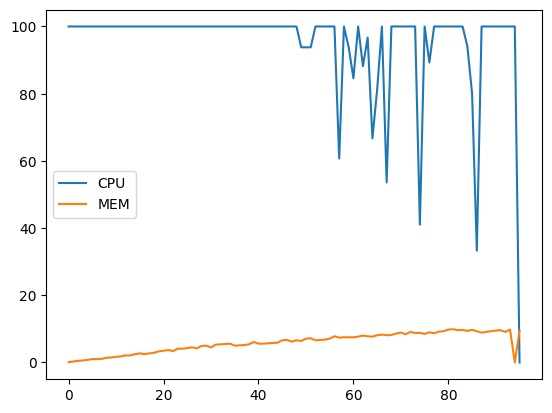
\includegraphics[scale=0.8]{graphs/11.png}
    \item 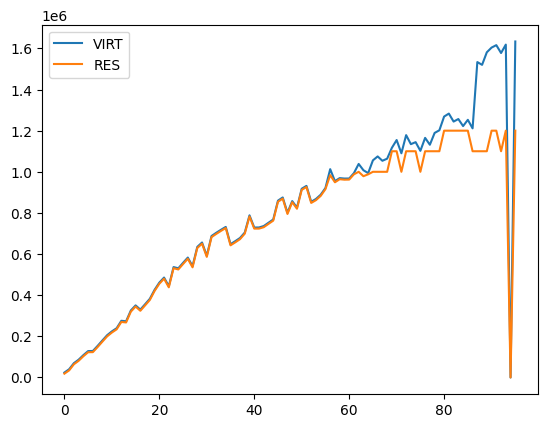
\includegraphics[scale=0.8]{graphs/12.png}
    \item 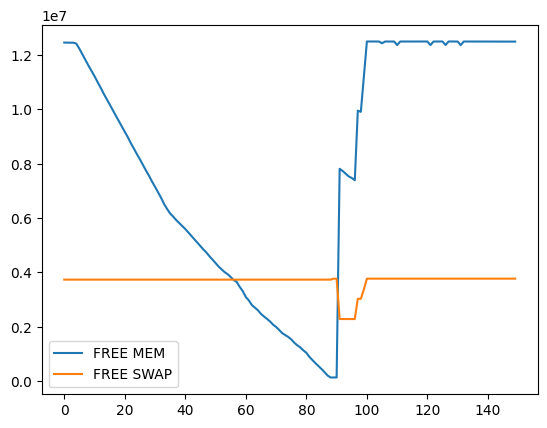
\includegraphics[scale=0.8]{graphs/13.png}
\end{itemize}

\textbf{Комментарий: }
Процесс аварийно не завершился, журнал пуст, весьма логично: в первом эксперименте размер массива как раз и был \texttt{20 800 000 * 10}. (Да, \texttt{free mem} обнулился, но использование swap продолжилось недолго и этого хватило.)

\subsubsection*{Рассмотрим \textbf{N = 20 800 000} \textbf{K = 30}}

\begin{itemize}
    \item 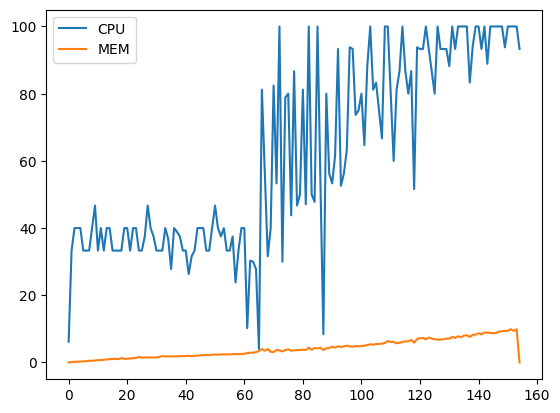
\includegraphics[scale=0.8]{graphs/14.png}
    \item 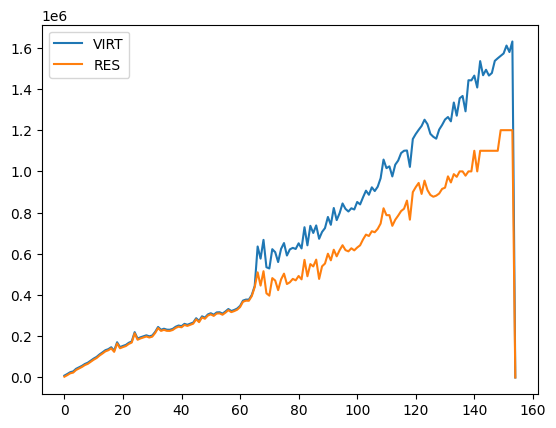
\includegraphics[scale=0.8]{graphs/15.png}
    \item 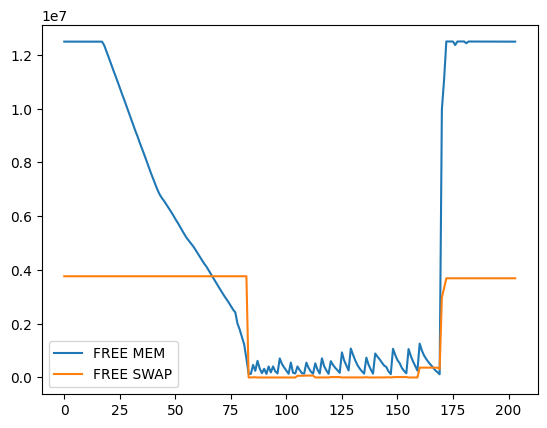
\includegraphics[scale=0.8]{graphs/16.png}
\end{itemize}

Результат \textbf{dmesg | grep "newmem.bash" } лежит в файле \texttt{dmesg1.log}.

\textbf{Комментарий: }
Процесс аварийно завершился. Потому что \texttt{20 800 000 * 30} $>$ \texttt{20 800 000 * 10}.

\subsubsection*{Рассмотрим \textbf{N = 7 000 000} \textbf{K = 30}}

\begin{itemize}
    \item 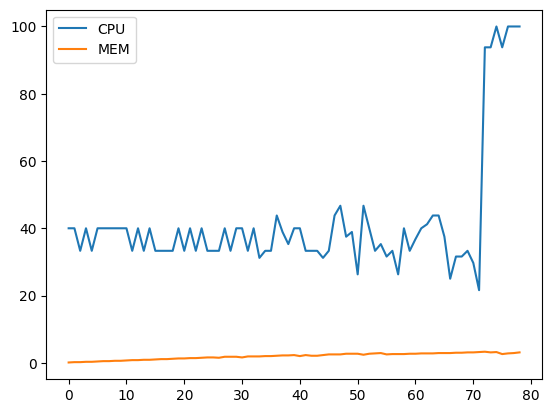
\includegraphics[scale=0.8]{graphs/17.png}
    \item 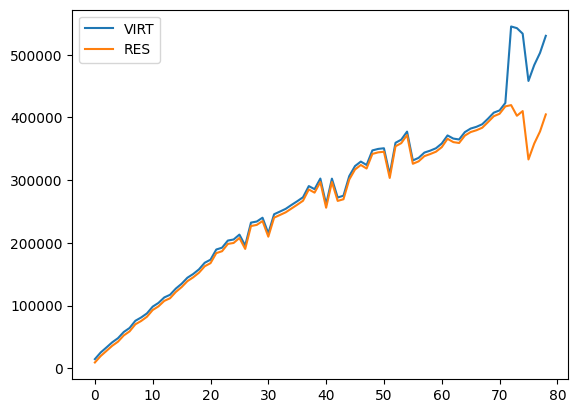
\includegraphics[scale=0.8]{graphs/18.png}
    \item 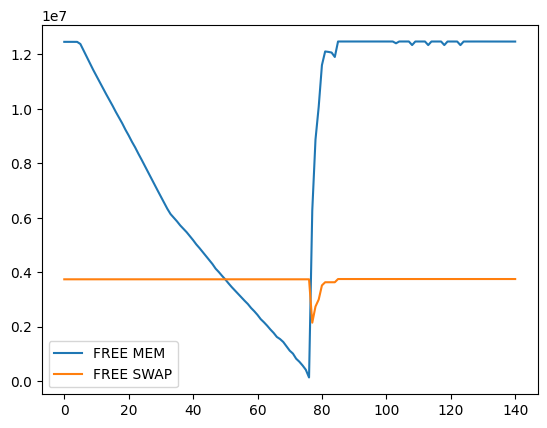
\includegraphics[scale=0.8]{graphs/19.png}
\end{itemize}

\textbf{Комментарий: }
Мы взяли \texttt{N = 7 000 000}, потому что \texttt{208 000 000 / 30 = 6 933 333.(3) $\approx$  7 000 000}. 
Процесс не завершился аварийно, журнал пуст.

\subsubsection*{Рассмотрим \textbf{N = 7 500 000} \textbf{K = 30}}

\begin{itemize}
    \item 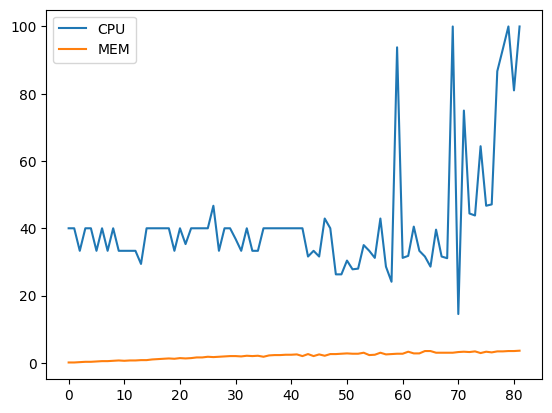
\includegraphics[scale=0.8]{graphs/23.png}
    \item 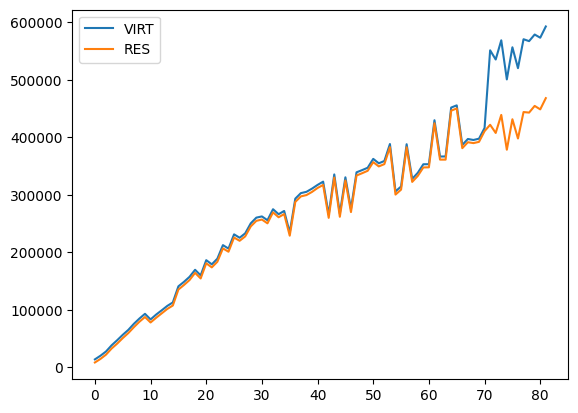
\includegraphics[scale=0.8]{graphs/24.png}
    \item 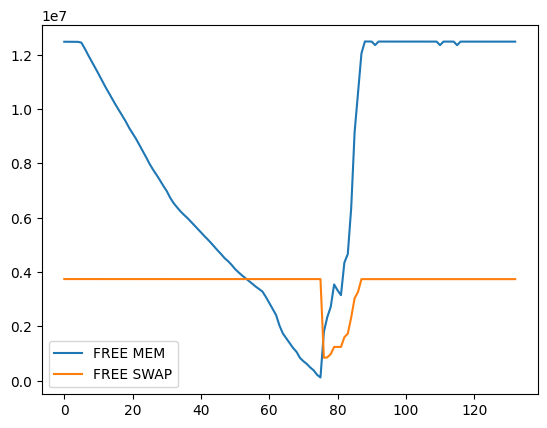
\includegraphics[scale=0.8]{graphs/25.png}
\end{itemize}
\textbf{Комментарий: }
Процесс не завершился аварийно, НО видно, что free swap стремится вниз. Максимальное значение N, чтобы при K=30 не происходило аварийных завершений процессов, существует при free swap, находящемся на $\varepsilon$ расстоянии от нуля.

\subsubsection*{Рассмотрим \textbf{N = 8 000 000} \textbf{K = 30}}

\begin{itemize}
    \item 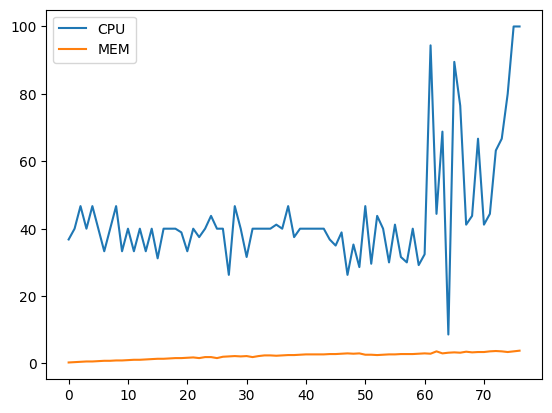
\includegraphics[scale=0.8]{graphs/20.png}
    \item 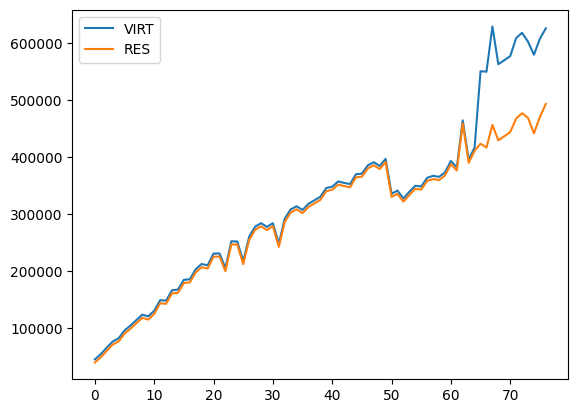
\includegraphics[scale=0.8]{graphs/21.png}
    \item 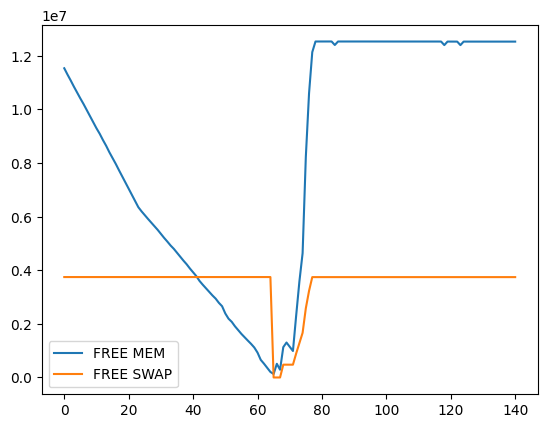
\includegraphics[scale=0.8]{graphs/22.png}
\end{itemize}

Результат \textbf{dmesg | grep "newmem.bash" } лежит в файле \texttt{dmesg2.log}.

\textbf{Комментарий: }
Процесс аварийно завершился.

\subsection*{Итоги второго эксперимента: }
\begin{itemize}
    \item При \texttt{N = 20 800 000}, \texttt{K = 10} всё круто.
    \item При \texttt{N = 20 800 000}, \texttt{K = 30} ряд процессов закончился аварийно, т.к. процессы требуют суммарно приблизительно в 3 раза больше оперативной памяти, чем доступно.
    \item Максимальное значение \texttt{N}, такое что при \texttt{K=30} не происходило аварийных остановок процессов $\approx 7.5 \cdot 10^6$ (если быть точнее: оно между $7.5$ и $8$). Оно отличается от ожидаемого значения --- \(2.08\cdot 10^8 / 30 \approx 7\cdot 10^6\), т.к. процессы не работают синхронно и некоторые достигают штатного завершения раньше других, пока оперативной памяти хватает.
\end{itemize}

\end{document}






